\documentclass[a4paper, 12pt]{book}

\usepackage[T1]{fontenc}
\usepackage[utf8]{inputenc}
\usepackage[italian]{babel}
\usepackage{graphicx}
\usepackage{sidecap}
\usepackage{subfig}
\usepackage[colorlinks]{hyperref}
\hypersetup{linktoc=all}


\begin{document}
    
\author{Giovanni Tosini}
\title{Sistemi Operativi \\
\large Secondo semestre}
\date{ }
\maketitle
\newpage
\tableofcontents
\newpage

\chapter{Monitor}

Si tratta di una struttura simile ai semafori, implementa di default la mutua esclusione. Simile a una classe di un linguaggio a oggetti, può contenere:
\begin{itemize}
    \item variabili(sono private)
    \item metodi(solo loro possono utilizzare le variabili definite all'interno del Monitor)
    \item costruttore
\end{itemize}

Quando un processo usa una entry del Monitor, gli altri non possono accedervi. Al suo interno posso dichiarare variabili di tipo CONDITION, non hanno valore, vengo usate esclusivamente con i metodi WAIT e SIGNAL.

\begin{verbatim}
    CONDITION x
    x.wait -> blocca il processo, non avvengono incrementi
              o decrementi come con i semafori
    x.signal -> se fatto quando non ci sono processi in
                attesa, non fa niente
\end{verbatim}

\begin{center}
    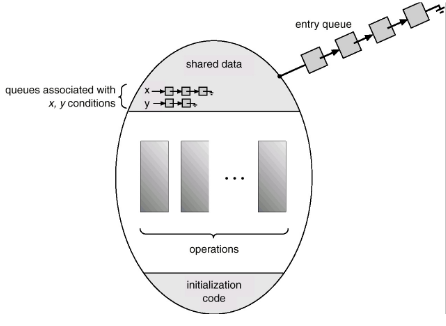
\includegraphics[width=0.5\textwidth]{ovetto.png}
\end{center}

Il comando SIGNAL può rompere la mutua esclusione, perché un eventuale processo fermo potrebbe ripartire e in quel caso entrambi sarebbe all'interno della sezione critica, per evitare ciò il processo che la chiama:
\begin{itemize}
    \item viene bloccato
    \item oppure SIGNAL deve essere l'ultima istruzione prima di uscire dal Monitor
\end{itemize}

Quale metodo usare? Dipende dal Monitor.

\section{Problematiche}

\begin{itemize}
    \item esistono pochi linguaggi che li implementano
    \item possono essere applicati solo quando ci sono processi che condividono la memoria(stessa macchina)
\end{itemize}

\chapter{Deadlock}

Causato quando un processo è in attesa di un evento causato a sua volta da un altro processo in attesa.
Ci sono quattro condizioni che possono causare un Deadlock:

\begin{itemize}
    \item mutua esclusione
    \item hold and wait: processo che detiene una risorsa ed è in attesa di una risorsa utilizzata da un altro
    \item no preemption: il processo deve rilasciare volontariamente la risorsa(non può essere ucciso)
    \item catena circolare: A attende B, che attende C, che attende A
\end{itemize}
In presenza di tutte e quattro esiste la possibilità che si verifichi.
Tecnica di prevenzione: basta che una delle quattro non venga rispettata e il Deadlock non può avvenire.

\paragraph{Modello astratto RAG (Resource Allocation Graph)}

\begin{center}
    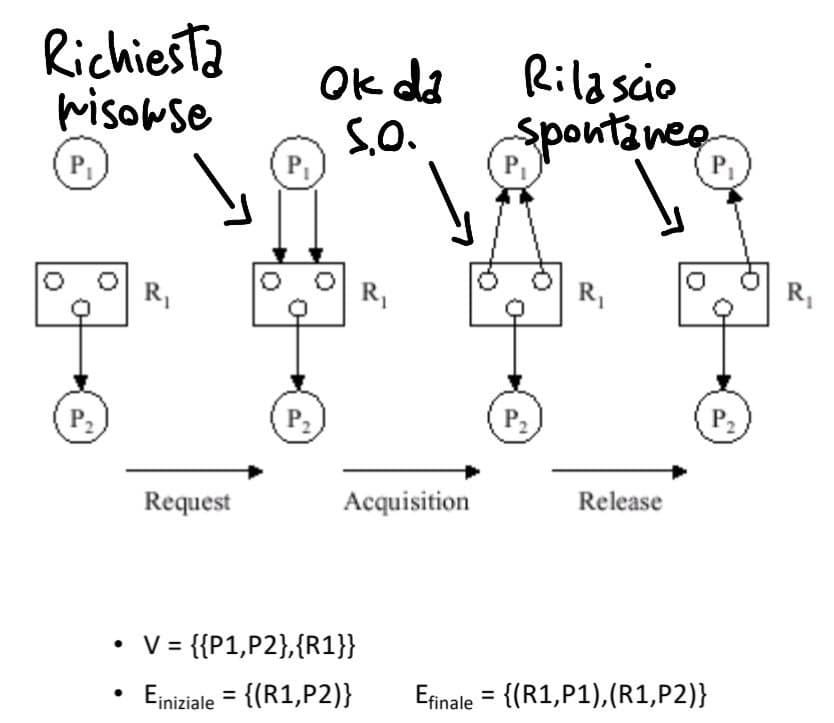
\includegraphics[width=0.5\textwidth]{rag.jpg}    
\end{center}
In generale, se abbiamo una sola istanza di ogni risorsa e siamo in presenza di un ciclo, il Deadlock è certo.
Con risorse con più istanze invece non è assicurato.

\section{Gestione Deadlock}

Prevenzione statica: evitare ovvero che si verifichino una della quattro condizioni sopra riportate,
se ci sono risorse disponibili non le assegno a prescindere.

\begin{itemize}
    \item mutua esclusione: non posso toglierla
    \item hold and wait: accumulo tutte le risorse tutte in una volta altrimenti non procedo
    questo porta a delle problematiche:
    \begin{itemize}
        \item basso uso delle risorse
        \item starvation
        \item occorre conoscere le risorse necessarie
    \end{itemize}
    \item no preemption: un processo che richiede una risorsa non disponibile
    sarà costretto a rilasciare tutte le altre risorse che stava tenendo
    \item ogni risorsa avrà una priorità crescente, il processo può richiederle esclusivamente in ordine crescente
\end{itemize}
Prevenzione dinamica, durante l'esecuzione si blocca un processo in base al RAG, occorre conoscere  a priori il caso peggiore 
in cui si causa un Deadlock e permette di sfruttare maggiormente le risorse per altri processi diversamente da quella statica.
Guardando il RAG, come un processo richiede una risorsa ipotizza di concederla e verifica se si presenta un ciclo,
in caso affermativo la richiesta verrà rifiutata, il processo rimarrà in attesa e il sistema resterà in 
un stato SAFE.

\vspace{3ex}
\begin{tabular}{|c|c|c|}
    \hline
    x & Richieste & Possedute \\
    \hline
    p0 & 10 & 5 \\
    \hline
    p1 & 4 & 2 \\
    \hline
    p2 & 9 & 2 \\
    \hline    
\end{tabular}

\vspace{3ex}p0 avrà bisogno di 10 istanze delle quali già ne possiede 5,12 sono quelle presenti, 9 in uso e 3 libere.
Stato SAFE o UNSAFE? Si va in ordine per processo:

\begin{itemize}
    \item p0 ne sta usando 5, ne occorrono altre 5, con le 3 libere non può essere soddisfatto, di conseguenza rimarrà in attesa
    \item p1 ne chiede 4, ne ha già 2, 3 sono libere, di conseguenza se andasse prima lui ne avremmo 5 libere dopo
\end{itemize}
Quindi saremmo in uno stato SAFE.\\
N.B.: lo scheduler in tutto ciò non ha rilevanza, lui si limita scegliere quali processi mettere nella CPU.

Lo svantaggio della
previsione dinamica è l'uso delle risorse minore, perché ci possono esserne alcune che non vengono sfruttate.

\vspace{3ex}1) L'algoritmo RAG funziona solo con risorse che possiedono un'unica istanza, funzionamento:

\begin{itemize}
    \item aggiungo al RAG l'arco di reclamo, ovvero in futuro quel processo richiederà l'uso di quella risorsa molto probabilmente
    \item il S.O. permetterà al processo di usare la risorsa solo se ipotizzando che venga fatto, non si verifichi un ciclo
\end{itemize}

\begin{center}
    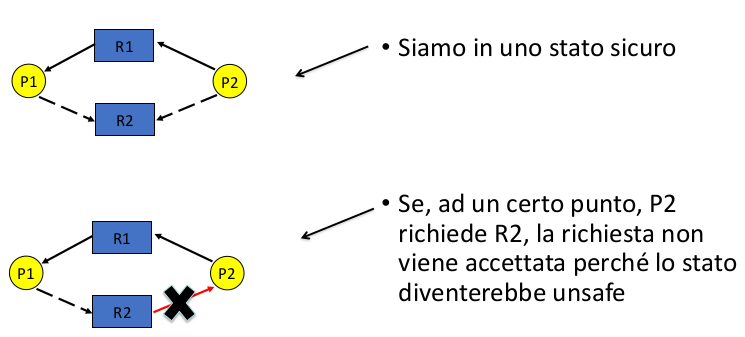
\includegraphics[width=0.8\textwidth]{rag_reclamo.png}
\end{center}
La freccia tratteggiata indica l'arco di reclamo.

2) L'algoritmo del banchiere è meno efficiente dell'algorimo RAG, ma
funziona con qualsiasi numero di istanze delle risorse. Si divide in due parti, una che simula la cessione dell'istanza della risorsa
e una che ne verifica l'effetto.

\begin{center}
    \includegraphics*[width=1\textwidth]{banchiere3.png}
\end{center}

\begin{center}
    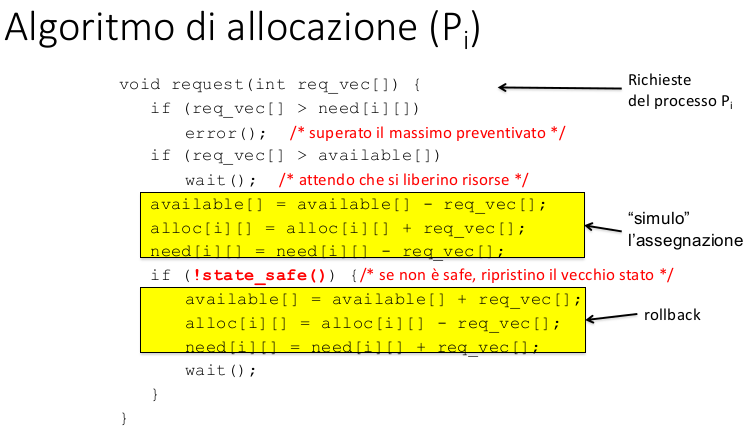
\includegraphics[width=1\textwidth]{banchiere1.png}
\end{center}

\begin{center}
    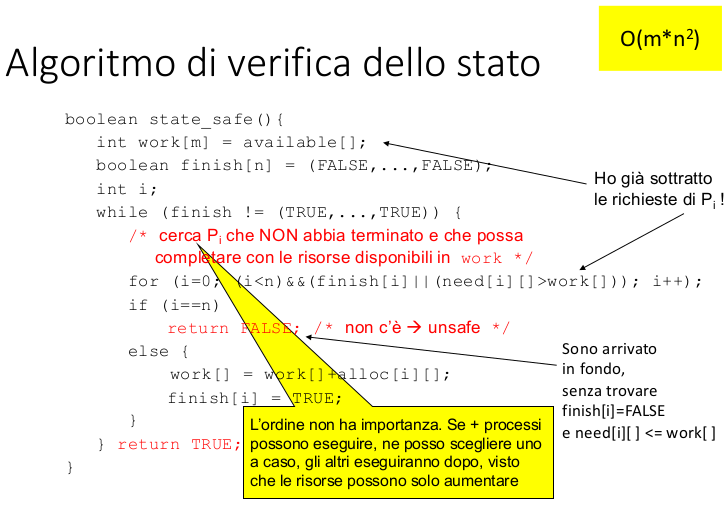
\includegraphics[width=1\textwidth]{banchiere2.png}
\end{center}
3) L'algoritmo di rilevazione permette che ci siano dei Deadlock, ogni tanto verifica che il sistema sia caduto in Deadlock
 in un metodo simile all'algoritmo del banchiere senza la necessità di conoscere la matrice max, verifica solo se il sistema è in 
 uno stato SAFE. Usa strutture dati simili a quello del banchiere.
 \begin{center}
     \begin{verbatim}
         int available[m]; //n° istanze di R_i disponibili
         int alloc[n][m]; //matrice allocazione corrente
         int req_vec[n][m]; //matrice di richiesta,
                            //stesse dimensione della max,
                            // è una max istantanea
     \end{verbatim}
 \end{center}
 \begin{center}
     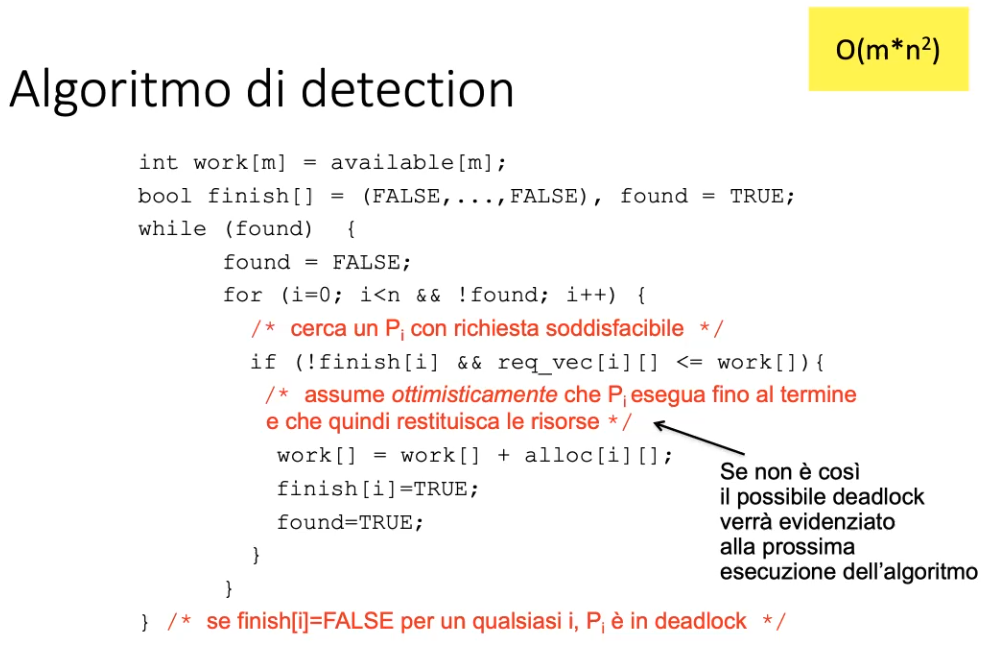
\includegraphics[width=1\textwidth]{detection.png}
 \end{center}
 Parte dal presupposto che tutti i processi siano bloccati,
 verifica se il singolo processo non ha finito e se le risorse che richiede siano inferiori a quelle disponibili.
  come trova un processo che può proseguire
  con la sua esecuzione significa che non si è in Deadlock, non verifica la situazione futura, solo quella attuale.
Esempio:
\begin{center}
    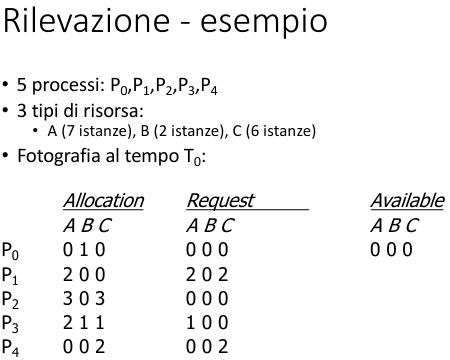
\includegraphics[width=1\textwidth]{detection2.png}
\end{center}
Usando l'algoritmo si passa man mano ogni singolo processo e si verifica se nello stato attuale può finire la sua esecuzione
 oppure è fermo a causa di un'attesa di risorse. Man mano che si trovano processi che possono concludere, si considerano 
 le risorse in loro possesso come possibili risorse future disponibili.

 L'algoritmo di rilevazione può essere lanciato:
 \begin{itemize}
     \item dopo ogni richiesta di risorsa
     \item ogni N secondi
     \item quando la percentuale di utilizzo della CPU cala sotto una soglia T
 \end{itemize}
 La prima è particolarmente costosa, non si fa prevenzione, ma si verifica sempre, che può essere problematico essendo 
 un algoritmo che può arrivare ad avere una complessità cubica. La terza opzione potrebbe non rilevare dei Deadlock causati da 
 piccoli gruppi di processi che non causano grossi cali d'uso della CPU.

 Quando ci si accorgerà del Deadlock si potrà:
 \begin{itemize}
     \item uccidere tutti o alcuni dei processi coinvolti
     \item prelazionare tutti i processi coinvolti
 \end{itemize}
 In entrambi i casi sarebbe un grosso danno, perché i processi hanno lavorato fino a quel momento  
 per niente.
 Per la prima, invece di uccidere tutti i processi si può scegliere di ucciderne uno alla volta in base a 
 alle risorse allocate, a quante ne mancano, a quanto tempo mancava, etc e verificare dopo se il Deadlock 
 è tuttora presente o meno.
 La seconda possibilità invece porta il problema che prelazione un singolo processo equivale quasi a ucciderlo 
 visto che non può continuare normalmente come prima, una possibile soluzione è il \textbf{rollback} che comporta
 un lavoro in precedenza eseguito dalla CPU per salvare uno stato in cui il processo non era bloccato.
 Successivamente quest potrebbe causare un fenomeno di starvation se si andrà a fare \textbf{rollback} dei soliti
 processi, in quel caso una possibile soluzione potrebbe essere quella di considerare il numero di \textbf{rollback}
 nei fattori di costo.

 \chapter{Gestione della memoria}

 Un processo ha bisogno sia di memoria RAM che di memoria di massa per poter lavorare. La memoria serve ai processi per
 via dell'uso del \textbf{Program Counter} da parte della CPU .
 Possono nascere svariati problemi nella gestione della memoria per i processi:
 \begin{itemize}
     \item l'allocazione della memoria dei singoli processi
     \item protezione dello spazio allocato
     \item condivisione dello spazio allocato
     \item gestione dello swap
     \item gestione della memoria virtuale
 \end{itemize}
 Ogni programma per essere eseguito deve essere messo in memoria e trasformato in processo, da quel momento la CPU
 preleverà istruzioni dalla memoria in base al \textbf{Program Counter}, questo può portare all'ulteriore prelievo di dati dalla
 memoria fino alla fine dell'esecuzione con l'eventuale scrittura in memoria del risultato, una volta che il processo terminerà
 la memoria verrà rilasciata.

 \paragraph{Come avviene il passaggio da programma a processo?}
 La trasformazione avviene tramite una trasformazione di indirizzi di memoria.
 \begin{center}
     \begin{verbatim}
         int x = 3;
     \end{verbatim}
 \end{center}
 non è altro che un riferimento a un indirizzo di memoria, quando il programma verrà eseguito, quell'indirizzo
 \textbf{simbolico} verrà tradotto in un indirizzo \textbf{fisico}.
 \paragraph{Chi compie questa trasformazione?}
 \begin{description}
     \item [il compilatore:] prende l'indirizzo \textbf{simbolico} e lo trasforma in una serie di indirizzi \textbf{rilocabili}
     ovvero che si possono posizionare da un'altra parte
     \item [il linker e/o il loader:] prendono l'indirizzo \textbf{rilocabile} e lo trasformano in indirizzo fisico assoluto
 \end{description}
 Possono essere coinvolti tutti o no, in base a come avviene la trasformazione.
 \begin{center}
     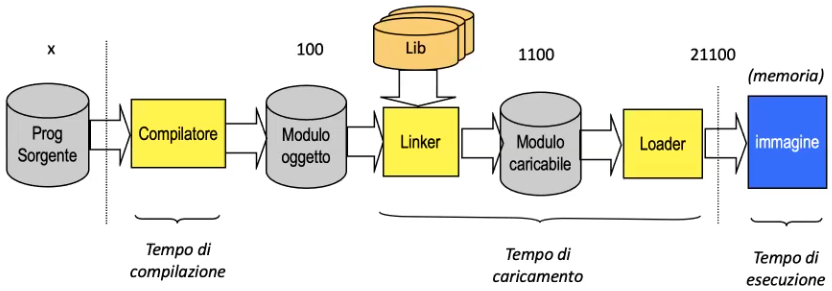
\includegraphics[width=1\textwidth]{trasformazione.png}
 \end{center}
La variabile X viene presa dal \textbf{compilatore} e trasformata da indirizzo \textbf{simbolico} a indirizzo \textbf{rilocabile}, viene
creato un modulo oggetto, in cui alla variabile viene assegnato un indirizzo di memoria, X non sarà più X, sarà l'area di memoria
all'indirizzo 100. Il \textbf{linker} collegherà l'indirizzo 100 con gli indirizzi delle eventuali librerie incluse nel programma,
ciò causerà la creazione di un modulo ricaribile in memoria. La X dall'indirizzo 100 sarà spostata all'indirizzo 1100 per fare spazio
alle eventuali librerie. Il modulo caricabile è quello che effettivamente verrà caricato in memoria dal \textbf{loader}. Il SO
assegnerà uno spazio all'interno della memoria tenendo conto dello spazio effettivamente occupato al momento. Eventualmente se
l'indirizzo 1100 fosse occupato, il SO potrà spostarlo a un altro indirizzo libero, fatto questo il processo verrà eseguito.
Se si troverà un'istruzione 
\begin{center}
    \begin{verbatim}
        int a = x + b;
    \end{verbatim}
\end{center}
vedendo che l'operando da prelevare è X, verrà ripescato dall'indirizzo di memoria, tale azione che collega indirizzi 
\textbf{simbolici} a indirizzi \textbf{fisici} viene denominata \textbf{binding degli indirizzi}.
\section{Tempi di compilazione}
\begin{description}
    \item[compile-time:] avviene a tempo di compilazione,in quel caso ci sarà solo il 
    \textbf{compilatore} che non può sapere se l'indirizzo che assegna al programma sia occupato o meno, di conseguenza 
    in caso in cui fosse occupato il programma semplicemente non verrà eseguito. Ciò funziona bene se la memoria è ottimizzata
    al massimo. Per cambiare la locazione del programma l'unica opzione sarà quellla di ricompilarlo.
    \item[load-time:]avviene a tempo di caricamento, il \textbf{loader} può notare che l'area di memoria in cui vuole
    caricare sia occupata e di conseguenza cambia l'area in cui andare a caricare. Il codice sarà rilocabile, anche se non permette
    di spostare il processo mentre è in esecuzione. Se cambiasse l'indirizzo di riferimento sarà necessario ricaricare.
    \item[run-time:]permette di spostare l'indirizzo di memoria allocato mentre il processo è in esecuzione, è necessario un 
    supporto hardware perché decisamente più efficiente. 
\end{description}
I primi due tipi di \textbf{binding} sono considerati \textbf{statici} mentre l'ultimo è considerato \textbf{dinamico}.

\section{Linking}

Può essere diverso indipendentemente dal tipo di \textbf{binding}.
\begin{description}
    \item[statico:] tradizionale, prima di mandare in esecuzione il processo, si è creato un'immagine di memoria con 
    tutte le librerie incluse.
    \item[dinamico:]il sistema viene preparato per accogliere un'immagine del codice e delle librerie, ma il linking vero e
    e proprio avverrà solo al momento dell'esecuzione, l'eseguibile sarà più piccolo perché non conterrà le librerie, ma solo 
    il loro riferimento.  
\end{description}

Un programma linkato staticamente occuperà una maggior memoria rispetto a un programma linkato dinamicamente, dal punto di vista
di caricamento il dinamico vince sullo statico, in quel caso gli stub creati dal linkato dinamico dovranno essere completati a 
\textbf{run-time} e ciò porterà il programma a essere più lento rispetto a quello linkato staticamente.

Ricapitolando:
\begin{description}
    \item[linking statico:]\begin{itemize}
        \item occupa maggior memoria
        \item lento nel caricamento
        \item veloce nell'esecuzione
    \end{itemize} 
    \item[linking dinamico:]\begin{itemize}
        \item occupa meno memoria
        \item più rapido nell'avvio
        \item più lento nell'esecuzione
    \end{itemize}
\end{description}

\section{Loading}

Lo stesso concetto di statico e dinamico può essere applicato al \textbf{loader}.
\begin{description}
    \item[statico:] tutto il codice viene caricato in memoria al tempo di esecuzione, quindi deve essere disponibile in 
    memoria prima di eseguire il programma
    \item[dinamico:] i moduli che servono al processo vengono caricati al primo utilizzo, se una parte non serve non verrà
    caricata di conseguenza 
\end{description}

Uno dei malus dello \textbf{statico} è la possibilità di programmi in cui una parte del codice non verrà mai eseguita (magari
per via di condizioni), non conviene di conseguenza caricare completamente il programma, in quel caso il loading \textbf{dinamico}
diventa decisamente più utile.

\section{Spazio di indirizzamento logico}

Consiste nello spazio visto dalla CPU quando esegue un processo, mappato su uno spazio di indirizzamento fisico in RAM. Il SO 
deve mappare indirizzi logici o virtuali su indirizzi fisici reali, quando si fa \textbf{binding} a \textbf{compile-time} o
\textbf{load-time} l'indirizzo logico e fisico coincidono. Invece con un \textbf{binding} a \textbf{run-time} l'indirrizzo
logico generato dalla CPU potrebbe non coincidere con quello fisico presente in RAM, tutto ciò viene sempre gestito dal
SO. Una gestione dinamica come questa ha un costo, ovvero il tempo che ci mette la MMU (Memory Management Unit) che tiene 
conto del riferimento tra indirizzo logico a quello fisico a tradurre la richiesta.

La MMU può essere composta da un registro e un sommatore che somma gli indirizzi logici con un offset, potrebbe essere problematico
con processi che dovrebbero essere divisi all'interno dello spazio di memoria.

\chapter{Schemi di gestione della memoria}

\section{Allocazione contigua}

L'immagine di memoria del processo sarà tutto allocata in un'area contigua per l'appunto, senza buchi in mezzo. Per gestire tale
l'allocazione in questo modo esistono delle varianti:

\subsection{Partizioni fisse}

La memoria è divisa a blocchi, ciascun blocco con una determinata
    dimensione che rimarrà fissa per sempre, tra di loro possono differire in dimensione, ma rimarranno fisse. Il processo che arriva
    verrà posizionato nella prima partizione che permette di contenerlo. Un contro è che se un blocco viene occupato solo in 
    parte, quella libera sarà sprecata, perché il blocco è fisso e non può essere partizionato. Esistono delle opzioni:

    \begin{itemize}
        \item un'unica coda di attesa, con i processi in fila e come si libera uno spazio il processo in testa verificherà
        se riesce a entrarci o meno
        \item tante code, una per partizione, il SO fa un preselezione del processo che verrà messo nella coda più adatta a lui
    \end{itemize}

    Entrambe hanno vantaggi e svantaggi, una coda per partizione causerà la possibilità di avere delle code vuote e altre piene, 
    in quel caso si avrebbe tanta memoria sprecata e pochi processi in coda. Va bene solo nel caso in cui il carico dei vari processi
    è ben distribuito e di varie dimensioni. Se tutte le code fossero piene, sarebbe ottimale per l'uso della memoria.

    Nell'alternativa con un'unica coda, la gestione sarà più complicata, perché un processo troppo grande per stare in partizioni
    troppo piccole rimarrebbe in attesa in caso di algoritmo FCFS, bloccando tutti gli altri processi dietro di lui che 
    potrebbero entrare nelle partizioni libere. Una scansione della coda quando si libera una partizione risolve il problema, ci 
    sono due varianti
    
    \begin{description}
        \item[Best-fit:] scansiona tutta la coda scegliendo quello più adatto alla partizione che si è liberata
        ovvero quello che si avvicina a occuparla maggiormente, se la coda è molto lunga il tempo impiegato sarà decisamente
        elevato;
        \item[Best-available-fit:] viene scelto il primo processo che può stare nella partizione che si è liberata, non minimizza
        lo spreco, perché potrebbe esserci un processo che occuperebbe meglio la partizione.
    \end{description}

Lo schema della MMU con un allocazione contigua a partizioni fisse è il seguente:

\begin{center}
    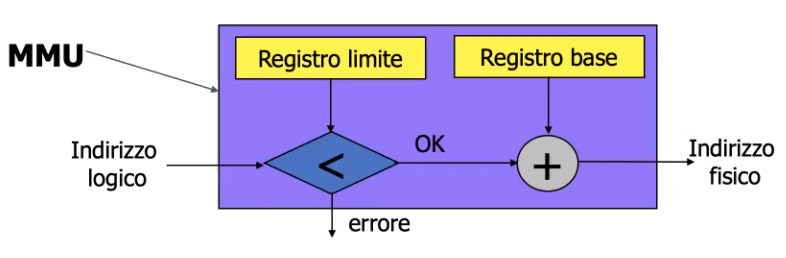
\includegraphics[width=1\textwidth]{mmu_partizioni_fisse.png}
\end{center}

Pro e contro:

\begin{description}
    \item[Pro:] semplicità, il SO deve solo tenere traccia di una tabella in cui si definisce in quale partizione andrà il processo
    \item[Contro:] il livello di multiprogrammazione è vincolato dal numero di partizioni, inoltre c'è uno spreco di memoria causato
    dalla frammentazione:
    
    \begin{description}
        \item[Interna:] causata dall'assegnamento di un processo a una partizione che non viene occupata al 100%
        \item[Esterna:] la somma della parte libera di partizioni parzialmente occupate potrebbe essere grande a sufficienza
        per un processo che invece sarà costretto ad attendere 
    \end{description}
    la frammentazione riduce l'efficacia nell'uso della memoria, la tecnica con partizioni fisse soffre di entrambe, è più adatta per
    processi delle dimensioni giuste ed esatte alle partizioni che si vogliono occupare, quindi più verso i sistemi embedded.
\end{description}

\subsection{Partizioni variabili}

Il processo che arriva in memoria si prenderà una fetta di memoria grande esattamente quanto lo spazio che occuperebbe.
La frammentazione esterne rimarrà, esempio:

\begin{itemize}
    \item si crea una partizione da 100, una da 50, una da 30 e una da 20
    \item si libera quella da 50 e da 20
    \item un processo che occupa 70 potrebbe entrare se le posizioni da 50 e 20 venissero sommate, ma non si può a causa dell'allocazione contigua
\end{itemize}

Si genera un effetto a "groviera". 
 
\subsection{Tecnica del Buddy System}

Un compromesso tra partizioni fisse e variabili, ovvero
ha partizioni fisse, ma anche variabili, le dimensioni 
non sono customizzate, ma non rimangono fisse. Bisogna 
immaginare la memoria un blocco fisso, come arriva un
processo parte il sequente schema:  

\begin{SCfigure}[50][h!]
    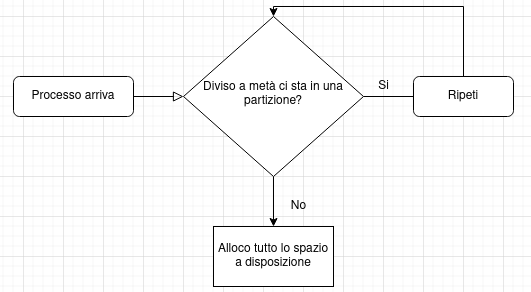
\includegraphics[width=0.5\textwidth]{buddy_system.png}
    \caption{Flowchart Buddy System}
\end{SCfigure}

Questo crea liste di blocchi liberi in base alla dimensione,
al processo successivo si andrà a guardare nella lista
se ci sta altrimenti si ripete la divisione.

\section{Paginazione}

Elimina totalmente la frammentazione esterna. La memoria fisica
viene suddivisa in tante piccole aree della stessa dimensione detti \textbf{frame}.
Lo spazio di allocazione non deve essere contiguo, al processo 
che arriva si daranno piccole aree fino a occupare tutte 
quelle necessarie. Il processo viene diviso,
quando un processo dovrà essere eseguito in CPU, SO dovrà
ricomporlo, quindi occorre una mappa delle locazioni.

La CPU è a conoscenza degli indirizzi logici, la memoria
logica viene divisa in blocchi della stessa dimensione le \textbf{pagine}, il SO 
trasforma le pagine in frame.
Entra in aiuto una tabella delle pagine, ovvero una mappa
della memoria specifica per ogni singolo processo, attraverso
la quale il SO riesce a tradurre l'indirizzo logico che serve alla 
CPU in un indirizzo fisico e recuperare di conseguenza le 
informazioni necessarie.

Esempio:
\begin{itemize}
    \item dimensione della pagina = 1KB
    \item dimensione del programma = 2.3KB
    \item saranno necessarie 3 pagine, dell'ultima si userà solo 0.3KB
\end{itemize}
Come si può notare sarà ancora possibile la frammentazione
interna.

\paragraph{Come avviene la ricerca nella tabella delle pagine?}
L'indirizzo logico richiesto dalla CPU è composto dal numero
di pagina e da un offset, SO tramite il numero di pagina 
andrà alla ricerca nella tabella delle pagine del processo
in questione, una volta trovato otterrà l'altra metà di 
indirizzo fisico da sommare all'offset per ottenere 
l'indirizzo fisico effettivo in memoria.

Ovviamente la tabella risiede in memoria, ed è come già detto 
specifica del processo. Nei registri della CPU sarà presente 
la locazione della tabella e anche la sua lunghezza, a ogni context 
switch tale valore viene aggiornato.

Questo causa un doppio accesso alla memoria: uno per 
la tabella delle pagine e uno per l'istruzione/dato necessari, per 
questo si usa una cache dedicata, \textbf{Translation look-aside table}(TLB), 
servirà a evitare il doppio accesso in memoria, in caso 
di cache miss, ovvero TLB non sarà in possesso della pagina, si 
dovrà per forza fare il doppio accesso in memoria.

Il costo effettivo di accesso in memoria sarà dato dalla 
somma del cache hit all'accesso in memoria:
\[
    \overbrace{(T_{MEM} + T_{TLB})\alpha\textrm{(parametro)}}^{\textrm{cache hit}} + \overbrace{(2T_{MEM} + T_{TLB})(1 - \alpha)}^{\textrm{accesso in memoria}}
\]

La tabella delle pagine è utile anche per altro:
\begin{description}
    \item[Bit di validità:] identifica se l'area di memoria 
    è stata mappata per il processo o no;
    \item[Caratteristiche:] un bit che comunica se la pagina
    è solamente leggibile o no, per esempio il codice di una programma
    è in sola lettura, oppure se la pagina sia eseguibile o meno.
\end{description}

\paragraph{Quanto è grande una tabella della pagine?}
La dimensione è stabilita in base alla memoria massima e alla configurazione,
ovvero quanto grande è ogni frame della memoria. In un ipotetico spazio di indirizzamento
virtuale grande $2^{64}$, se ogni pagina avesse una dimensione di 4KB ovvero $2^{12}$ potrei 
avere un numero di frame in memoria corrispondente al rapporto tra la memoria indirizzabile totale e
la dimensione della singola pagina. 
\[
    2^{64} / 2^{12} = 2^{52}
\]
Un numero decisamente enorme che occuperebbe una grossa fetta della RAM da moltiplicare per il 
numero di processi attivi. Si possono usare due metodi per evitare ciò:
\begin{itemize}
    \item una tabella delle pagine invertita;
    \item oppure la paginazione multilivello.
\end{itemize}

\subsection{Tabella delle pagine invertita}
Una tabella unica nel sistema e non per processo, indicizzata per frame che contiene:
\begin{itemize}
    \item l'indirizzo virtuale della pagina che occupa quel frame
    \item informazioni sul processo che usa la pagina
\end{itemize}
Il tempo di traduzione degli indirizzi cresce perché non sarà più una ricerca per indice, ma per contenuto. Perché 
la tabella è indicizzata per frame, mentre la CPU richiederà per pagina, il SO dovrà scorrere la tabella alla ricerca della 
pagina e solo così otterrà il frame corrispondente che sarà l'indice del contenuto. Questo viene facilitato tramite una struttura 
a tabella hash, invece di usare una ricerca lineare. Cambia come viene generato l'indirizzo richiesto dalla CPU, sarà diviso in tre parti:
\begin{itemize}
    \item offset;
    \item numero di pagina;
    \item PID del processo.
\end{itemize}

Con il numero di pagina e il PID ho la chiave per la tabella hash, così da ottenere il valore ricercato per la traduzione ovvero
l'indice, perché la tabella è indicizzata per frame!

\subsection{Paginazione multilivello}
Viene paginata anche la tabella delle pagine, quindi spezzettata per fare in modo che alcuni pezzi non siano in RAM, lasciando 
spazio libero in memoria per altro di più utile. Questa azione può essere ripetuta anche per i pezzi delle tabella delle pagine, 
per più livelli di paginazione.  Esempio:
\begin{itemize}
    \item indirizzo logico a 32 bit;
    \item dimensione della pagina = 4K = $2^{12}$;
    \item 12 bit per offset(d);
    \item 20 bit per numero di pagina:
    \begin{itemize}
        \item 10 bit per l'indice della tabella delle pagine esterna;
        \item 10 bit per l'offset all'interno della pagina della tabella delle pagine interna.
    \end{itemize}
\end{itemize}
Il costo per un accesso in memoria con una paginazione multilivello cambia di conseguenza nello speficico,
l'accesso in memoria sarà moltiplicato per $n + 1$ livelli di paginazione:
\[
    (T_{MEM} + T_{TLB})\alpha + ((n + 1)T_{MEM} + T_{TLB})(1 - \alpha)
\]
Il $+1$ causato dall'accesso al dato.

\section{Segmentazione}
Il problema della paginazione è che lo spezzettare a blocchi il processo viene fatto senza rispettare la struttura dati 
creata dal compilatore, sarebbe più utile avere pagine contenenti blocchi interi utili: una pagina con il main, una per le 
funzioni, etc\dots Finché la pagina ha una dimensione fissa questo non si può ottenere, la \textbf{segmentazione} è analoga alla 
paginazione, ma non si vincola più alla dimensione di una pagina fissa. Dal punto di vista di SO, avremo una tabella dei segmenti 
che verranno tagliati a dimensione variabile. Un segmento di dimensioni variabili torna ad avere la problematica dell'allocazione 
contigua, ovvero che non può essere messo dovunque, ma in blocchi unici. Nella tabella dei segmenti, ogni entry conterrà oltre 
che all'indirizzo base del segmento anche la sua dimensione, che precedentemente non era necessaria con le pagine. 
\paragraph{Come cambia la traduzione?}
La CPU richiederà un indirizzo composto da una parte segmento e una parte offset, l'offset verrà analizzato, per verificare se 
va oltre la dimensione del segmento o se rimane al suo interno (ecco da cosa viene causato il segmentation fault). La parte di offset
verrà sommata al valore restituito dalla tabella dei segmenti, che ricordiamo contenere la dimensione del segmento e la base da sommare
eventualmente all'offset. Esempio di traduzione:
\begin{center}
    \begin{tabular}{| c | c | c |}  
        \hline
        Segmento & Limite & Base \\
        \hline
        0 & 600 & 219 \\
        \hline
        1 & 14 & 2300 \\
        \hline
        2 & 100 & 90 \\
        \hline
        3 & 580 & 1327 \\
        \hline      
    \end{tabular}
\end{center}

A ogni segmento si avrà appunto il suo limite e la sua base, per esempio

\begin{itemize}
    \item se venisse richiesto il segmento $0$ e l'offset $430$ 
    si controlla il segmento $0$, si nota che l'offset $430$ è all'interno del limite di conseguenza l'indirizzo fisico sarà dato da: 
    offset + base = $649$.
    \item segmento $1$ offset $20$? segmentation fault perché $20$ è superiore al limite $14$
\end{itemize} 

La segmentazione mi garantisce di gestire ancora meglio tutti gli aspetti visti nella paginazione, perché adesso avrò la certezza
che il contenuto del segmento sarà omogeneo.

\paragraph{Svantaggi della segmentazione}

Torna il problema della frammentazione esterna, la pagina può essere messa in qualunque spazio, perché sono tutti uguali, 
mentre il segmento essendo variabile ma richiedendo un'allocazione contigua non può e ciò causa la frammentazione esterna. 
Una possibile soluzione al problema è l'unione della paginazione e della segmentazione, segmento il processo e ogni segmento lo 
pagino, segmentandolo prima mantengo l'unità logica che verrà paginata omogeneamente in multilivelli.

\section{Paginazione vs Segmentazione}

Vantaggi della paginazione:
\begin{itemize}
    \item non esiste frammentazione, a parte una piccola frammentazione interna;
    \item l'allocazione dei frame non richiede algoritmi specifici;
\end{itemize} 
Svantaggi della paginazione:
\begin{itemize}
    \item non mantiene l'omogeneità;
\end{itemize}
Vantaggi della segmentazione:
\begin{itemize}
    \item omogeneità;
    \item associazione di protezione/condivisione ai segmenti;
\end{itemize} 
Svantaggi della segmentazione:
\begin{itemize}
    \item richiede degli algoritmi di allocazione dinamica dello spazione, essendo i segmenti variabili;
    \item reintroduce la problematica della frammentazione esterna;
\end{itemize}

Unendole si porteranno dietro i vantaggi di ciascuna limitando gli svantaggi.

\section{Segmentazione paginata}

L'indirizzo logico sarà composto da segmento e offset, il numero di segmento verrà sommato al valore all'interno \textbf{Segment Table Base Register} (indica dove si trova la tabella dei segmenti all'interno della memoria) 
per andare a indicizzare la tabella dei segmenti. All'interno della tabella dei segmenti si troverà la lunghezza del segmento e 
la \textbf{Page Table Base} in cui si troverà l'indirizzo di locazione della tabella delle pagine specifica di quel segmento. 
L'indirizzo verrà combinato con l'offset, che è composto da due parti, una che indica il numero di pagina e una che indica 
l'offset effettivo. Il numero di pagina verrà sommata al \textbf{Page Table Base Register} per recuperare la riga effettiva della 
tabella delle pagine, una volta indicizzata la riga in questione, si sommerà il valore del frame all'offset effettivo e si farà 
l'accesso alla memoria per recuperare il dato necessario. 

\chapter{Memoria virtuale}

\section{Motivazioni}

L'immagine di memoria di un processo è davvero necessaria che sia \textbf{tutta} caricata in RAM? In generale no, serve solo una parte,
ovvero quella che rappresenta la località spazio temporale necessaria. Quella che non serve verrà lasciata sul disco, 
questo permetterà di lasciare spazio libero in memoria per altre immagini di memoria più utili e avvantaggiare la multiprogrammazione.
Lo spazio logico sarà più grande dello spazio in memoria, perché sarà composto dalla somma di tutte le immagini dei processi che 
saranno in parte in RAM e in parte sul disco. 

\section{Paginazione su domanda}

Una pagina si troverà in memoria solo quando necessaria. I vantaggi sono i seguenti:
\begin{itemize}
    \item meno memoria occupata da ogni processo;
    \item se il livello di multiprogrammazione fosse troppo alto, l'eventuale swap out verrà fatto solo a una parte delle pagine riucendo i tempi di I/O;
\end{itemize}

Per poter implementare occorre sapere se la pagina richiesta dalla CPU sia valida o no, entra in gioco il bit di validità presente
nella tabella delle pagine. Quel bit segnalerà se la pagina si trova in RAM, su disco oppure se la pagina non si trova 
nell'intervallo di memoria. Quando una pagina è mappata su un frame che non si trova in RAM, bit validità = 0, avviene un \textbf{page fault}.
Quindi:

\begin{enumerate}
    \item controllando sulla tabella delle pagine risulterà che la pagina è invalida, non è in RAM, di conseguenza sarà su disco;
    \item parte un interrupt, il \textbf{page fault};
    \item il S.O. verificherà che la pagina si trovi nella parte di disco dedicata alla funzione di RAM, (\textbf{Backing Store} o \textbf{Area di Swap});
    \item localizza la pagina e la riporta nella memoria, cercherà un frame e caricherà la parte di memoria recuperata;
    \item reset della \textbf{page table} per indicare che ora la pagina è in memoria con annessa aggiunta dell'indirizzo e modifica del bit validità;
    \item il processo verrà rimesso in ready queue per essere pronto all'esecuzione.
\end{enumerate}

Questo avviene a ogni \textbf{page fault}. 

\subsection{EAT di un Page Fault}

Introduciamo un parametro p (tasso di page fault), che vale in questo intervallo $0 \le p \le 1$, dove 

\begin{itemize}
    \item p = 0, nessun page fault;
    \item p = 1, ogni acceso è un page fault.
\end{itemize}

\[
    EAT = (1 - p) * t_{mem} + p * t_{\textrm{page fault}}
\]

La parte $p * t_{\textrm{page fault}}$ è la moltiplicazione tra la percentuale di page fault e il tempo richiesto per recuperare il 
dato su disco, mentre $t_{mem}$ è il tempo di accesso alla memoria tramite il meccanismo di gestione dell'allocazione di 
memoria ai processi. Il $t_{\textrm{page fault}}$ è composto dalla gestione dell'interrupt che arriva, il context switch per 
permettere al S.O. di gestire la situazione, torna al processo che era stato interrotto (context switch).

\begin{itemize}
    \item gestione dell'interrupt (primo context switch);
    \item swap in, lettura della pagina mancante da disco a memoria;
    \item costo di riavvio del processo (secondo context switch);
    \item (opzionalmente) swap out della pagina che devo estrarre per fare spazio a quella richiesta.
\end{itemize}

Ci sono ben due context switch.

\subsection{Rimpiazzamento delle pagine}

In caso di assenza di frame liberi in cui mettere la pagina recuperata:

\begin{itemize}
    \item tramite un algoritmo specifico di rimpiazzamento delle pagine si trova una pagina da sostituire;
    \item avviene lo swap su disco della pagina sostituita;
    \item swap dell'altra pagina nel frame dal disco;
    \item modifica le tabelle (tabella delle pagine e bit di validità);
    \item ripristino dell'istruzione che ha causato il page fault.
\end{itemize}

Rimpiazzare una pagina costa il doppio di una normale gestione del page fault. Per questo entra in gioco l'utilità del \textbf{dirty bit}
ovvero un bit che specifica se la pagina è stata modificata mentre si trovava in memoria o meno, in caso di una modifica occorre
ricaricarla su disco. Rimpiazzare una pagina che non è stata modifica costa meno, perché si può semplicemente sovrascrivere.

\subsection{Algoritmi di rimpiazzamento delle pagine}

Obiettivo: minimizzare il tasso di page fault, dipenderà dalla scelta delle pagine da caricare in memoria. Un metodo è l'uso 
di una stringa di riferimenti. Ipotizzando pagine grandi 100 byte, la stringa sarà composta dalla cifra delle centinaia delle 
pagine che verranno richieste. Esempio: 

\begin{itemize}
    \item indirizzi generati: 100, 604, 128, 130, 256, 260, 264, 268;
    \item la stringa di riferimento sarebbe composto da: 1, 6, 1, 1, 2 ,2, 2, 2;
    \item in realtà sarà composta da: 1, 6, 1, 2. Perché il page fault sarà possibile con la prima pagina, sicuramente non con quelle successive.
\end{itemize}

\subsubsection{Algoritmo FIFO}

Prima pagina che carico sarà la prima scelta a essere rimossa per liberare  eventualmente spazio, non è adatto nè per lo scheduling 
nè per la gestione della memoria. Può causare l'anomalia di Belady, ovvero aumentando la disposizione di frame in memoria potrebbero 
aumentare i page fault diversamente da quello che ci si aspetterebbe.






\end{document}